\title{Grunnatriði}
\author{Bergur Snorrason}
\date{\today}

\begin{document}

\frame{\titlepage}

\env{frame}
{
	\frametitle{Grunntög og takmarkanir þeirra}
	\env{itemize}
	{
		\item<1-> Í grunninn snýst forritun um gögn.
		\item<2-> Þegar við forritum flokkum við gögnin okkar með \emph{tögum}.
		\item<3-> Dæmi um tög í \texttt{C/C++} eru \texttt{int} og \texttt{double}.
		\item<4-> Helstu tögin í \texttt{C/C++} eru (yfirleitt):
		\item<5->[]
		\env{tabular}
		{
			{l l l}
			Heiti & Lýsing & Skorður\\
			\texttt{int} & Heiltala & Á bilinu $[-2^{31}, 2^{31} - 1]$\\
			\texttt{unsigned int} & Heiltala & Á bilinu $[0, 2^{32} - 1]$\\
			\texttt{long long} & Heiltala & Á bilinu $[-2^{63}, 2^{63} - 1]$\\
			\texttt{unsigned long long} & Heiltala & Á bilinu $[0, 2^{64} - 1]$\\
			\texttt{double} & Fleytitala & Takmörkuð nákvæmni\\
			\texttt{char} & Heiltala & Á bilinu $[-128, 127]$\\
		}
	}
}

\env{frame}
{
	\frametitle{Hvað með tölur utan þessa bila?}
	\env{itemize}
	{
		\item<1-> Einn helsti kostur \texttt{Python} í keppnisforritun er að heiltölur geta verið eins stórar (eða litlar) og vera skal.
		\pause \code{code/fact.py}
		\pause \code{code/fact.out}
		\item<4-> Það er einnig hægt að nota \texttt{fractions} pakkann í \texttt{Python} til að vinna með fleytitölur án þess að tapa nákvæmni.
	}
}

\env{frame}
{
	\frametitle{Hvað með tölur utan þessa bila?}
	\env{itemize}
	{
		\item<1-> Sumir \texttt{C/C++} þýðendur bjóða upp á gagnatagið \texttt{\_\_int128} (til dæmis \texttt{gcc}).
		\item<2-> Þetta tag býður upp á að nota tölur á bilinu $[-2^{127}, 2^{127} - 1]$.
		\item<3-> Þetta þarf ekki að nota oft.
	}
}

\env{frame}
{
	\frametitle{Röðun}
	\env{itemize}
	{
		\item<1-> Við munum reglulega þurfa að raða gögnum í einhverja röð.
		\item<2->[]
		\env{tabular}
		{
			{l l}
			Forritunarmál & Röðun\\
			\hline
			\texttt{C} & \texttt{qsort(...)}\\
			\texttt{C++} & \texttt{sort(...)}\\
			\texttt{Python} & \texttt{this.sort()} eða \texttt{sorted(...)}\\
		}
		\item<3-> Skoðum nú hvert forritunarmál til að sjá nánar hvernig föllin eru notuð.
	}
}

\env{frame}
{
	\frametitle{Röðun í \texttt{C++}}
	\env{itemize}
	{
		\item<1-> Í grunninn tekur \texttt{sort(...)} við tveimur gildum.
		\item<2-> Fyrra gildið svarar til fyrsta staks þess sem við viljum raða og seinna gildið vísar á enda þess sem við viljum raða
			(ekki síðasta stakið)
		\item<3-> Ef við erum með $n$ staka fylki \texttt{a} þá röðum við því með \texttt{sort(a, a + n)}.
		\item<4-> Við getum raðað flest öllum ílátum með \texttt{sort}.
		\item<5-> Ef við erum með eitthvað ílát (til dæmis \texttt{vector}) \texttt{a} má raða með \texttt{sort(a.begin(), a.end())}.
		\item<6-> Við getum líka bætt við okkar eigin samanburðarfalli sem þriðja inntak.
		\item<7-> Það kemur þá í stað ``minna eða samasem'' samanburðarins sem er sjálfgefinn.
	}
}

\env{frame}
{
	\frametitle{Röðun í \texttt{Python}}
	\env{itemize}
	{
		\item<1-> Til að raða lista í \texttt{Python} þá má nota annað hvort \texttt{this.sort()} eða \texttt{sorted(...)}.
		\item<2-> Gerum ráð fyrir að listinn okkar heiti \texttt{a}.
		\item<3-> Þá nægir að kalla á \texttt{a.sort()} og eftir það er \texttt{a} raðað.
		\item<4-> Hinsvegar skilar \texttt{sorted(a)} afriti af \texttt{a} sem hefur verið raðað.
		\item<5-> Til að raða \texttt{a} á þennan hátt þarf \texttt{a = sorted(a)}.
		\item<6-> Nota má inntakið \texttt{key} til að raða eftir öðrum samanburðum.
		\item<7-> Það er einnig inntak sem heitir \texttt{reverse} sem er Boole gildi sem leyfir auðveldlega að raða öfugt.
	}
}

\env{frame}
{
	\frametitle{Röðun í \texttt{C}}
	\env{itemize}
	{
		\item<1-> Í \texttt{C} er enginn sjálfgefinn samanburður, svo við þurfum alltaf að skrifa okkar eigið samanburðarfall.
		\item<2-> Til röðunar notum við fallið \texttt{qsort(...)}.
		\item<3-> Fallið tekur fjögur viðföng:
		\env{itemize}
		{
			\item<4-> \texttt{void* a}. Þetta er fylkið sem við viljum raða.
			\item<5-> \texttt{size\_t n}. Þetta er fjöldi staka í fylkinu sem \texttt{a} svarar til.
			\item<6-> \texttt{size\_t s}. Þetta er stærð hvers staks í fylkinu okkar (í bætum).
			\item<7-> \texttt{int (*cmp)(const void *, const void*)}. Þetta er samanburðarfallið okkar.
		}
		\item<8-> Síðasta inntakið er kannski flókið við fyrstu sýn en er einfalt fyrir okkur að nota.
		\item<9-> Þetta er \emph{fallabendir} (e. \emph{function pointer}) ef þið viljið kynna ykkur það frekar.
	}
}

\env{frame}
{
	\frametitle{Röðun í \emph{C}}
	\code{code/sort.c}
}

\env{frame}
{
	\frametitle{Uppsetning dæma}
	\env{itemize}
	{
		\item<1-> Dæmin sem við sjáum á Kattis eru (oftast) af stöðluðu sniði.
		\env{itemize}
		{
			\item<2-> Saga.
			\item<3-> Dæmið.
			\item<4-> Inntaks -og úttakslýsingar.
			\item<5-> Sýnidæmi.
		}
		\item<6-> Fyrstu tveir punktarnir geta verið blandaðir saman.
		\item<7-> Þeir eru líka lengsti hluti dæmisins.
	}
}
\env{frame}
{
	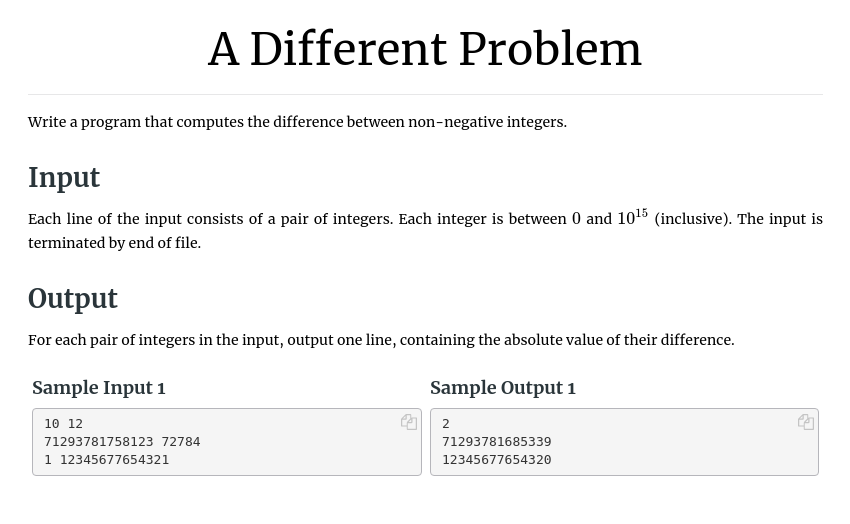
\includegraphics[scale = 0.38]{fig/daemi}
}

\env{frame}
{
	\frametitle{Röng lausn. Hver er villan?}
	\code{code/differentint.cpp}
}

\env{frame}
{
	\frametitle{Rétt lausn}
	\code{code/different.cpp}
}

\env{frame}
{
	\frametitle{\texttt{long long}}
	\env{itemize}
	{
		\item<1-> Við getum notað \texttt{typedef} til að spara okkur skriftir.
		\item<2-> Við bætum við \texttt{typedef <gamla> <nýja>;} ofarlega í skrána.
		\item<3-> Venjan í keppnisforritun er að nota \texttt{typedef long long ll;}.
		\item<4-> Við munum nota \texttt{typedef} aftur í námskeiðinu.
	}
}

\env{frame}
{
	\frametitle{Rétt lausn með \texttt{typedef}}
	\code{code/differentll.cpp}
}

\env{frame}
{
	\frametitle{\texttt{Time Limit Exceede}}
	\env{itemize}
	{
		\item<1-> Hvernig vitum að lausnin okkar sé of hæg?
		\item<2-> Ein leið er að útfæra lausnina, senda hana inn og gá hvað Kattis segir.
		\item<3-> Það myndi þó spara mikla vinnu ef við gætum svarað spurningunni án þess að útfæra.
		\item<4-> Einnig gæti leynst önnur villa í útfærslunni okkar sem gefur okkur \texttt{Time Limit Exceeded} (\texttt{TLE}).
		\item<5-> Til að ákvarða hvort lausn sé nógu hröð þá notum við \emph{tímaflækjur}.
		\item<6-> Sum ykkar þekkja tímaflækjur en önnur kannski ekki.
		\item<7-> Skoðum fyrst hvað tímaflækjur eru í grófum dráttum.
	}
}

\env{frame}
{
	\frametitle{Tímaflækjur í grófum dráttum}
	\env{itemize}
	{
		\item<1-> Keyrslutími forrits er háður stærðinni á inntakinu.
		\item<2-> Tímaflækjan lýsir hvernig keyrslutími forritsins eykst þegar inntakið stækkar (í versta falli).
		\item<3-> Ef forritið er með tímaflækju $\mathcal{O}(f(n))$ þýðir það að keyrslutíminn vex eins og $f$ þegar $n$ vex.
		\item<4-> Til dæmis ef forritið hefur tímaflækju $\mathcal{O}(n)$ þá tvöfaldast keyrslutími þegar inntakið tvöfaldast.
		\item<5-> Til annars dæmis ef forritið hefur tímaflækju $\mathcal{O}(n^2)$ þá \onslide<6->{fjór}faldast keyrslutími þegar inntakið tvöfaldast.
		\item<7-> Við ráð fyrir að grunnaðgerðirnar okkar taki fastann tíma, eða séu með tímaflækju $\mathcal{O}(1)$.
	}
}

\env{frame}
{
	\env{itemize}
	{
		\item<1-> Ef forritið okkar þarf að framkvæma $\mathcal{O}(f(n))$ aðgerð $m$ sinnum þá er tímaflækjan $\mathcal{O}(m \cdot f(n))$.
		\item<2-> Þetta er reglan sem við notum oftast í keppnisforritun.
		\item<3-> Hún segir okkur til dæmis að tvöföld \texttt{for}-lykkja, þar sem hver \texttt{for}-lykkja er $n$ löng, er
			$\mathcal{O}($\onslide<4->{$n^2$}$)$.
		\item<5-> Ef við erum með tvær einfaldar \texttt{for}-lykkjur, báðar af lenged $n$, þá er forritið 
			$\mathcal{O}(n + n) = \mathcal{O}($\onslide<6->{$n$}$)$
		\item<7-> Einnig gildir að tímaflækja forritsins okkar takmarkast af hægasta hluta forritsins.
		\item<8-> Til dæmis er
			$\mathcal{O}(n + n + n + n + n^2) = \mathcal{O}($\onslide<9->{$n^2$}$)$.
	}
}

\env{frame}
{
	\frametitle{Stærðfræði}
	\env{itemize}
	{
		\item<1-> Við segjum að fall $g(x)$ sé í menginu $\mathcal{O}(f(x))$ ef til eru rauntölur $c$ og $x_0$ þannig að
		\[
			|g(x)| \leq c \cdot f(x)
		\]
		fyrir öll $x > x_0$.
		\item<2-> Þetta þýðir í raun að fallið $|g(x)|$ verður á endanum minna en $k \cdot f(x)$.
		\item<3-> Þessi lýsing undirstrikar betur að $f(x)$ er efra mat á $g(x)$, og er því að segja að $g(x)$ hagi sér ekki verr en $f(x)$.
	}
}

\env{frame}
{
	\frametitle{Þekktar tímaflækjur}
	\env{itemize}
	{
		\item<1-> Tímaflækjur algrengra aðgerða eru:
		\item<2->[]
		\scriptsize
		\env{tabular}
		{
			{l | l | l}
			Aðgerð & Lýsing & Tímaflækja\\
			\hline
			Línulega leit & Almenn leit í fylki & $\mathcal{O}(n)$\\
			Helmingunarleit & Leit í röðuðu fylki & $\mathcal{O}(\log n)$\\
			Röðun á heiltölum & Röðun á heiltalna fylki & $\mathcal{O}(n \log n)$\\
			Strengjasamanburður & Bera saman tvo strengi af lengd $n$ & $\mathcal{O}(n)$\\
			Almenn röðun & Röðun með $\mathcal{O}(T(m))$ samanburð & $\mathcal{O}(T(m) \cdot n \log n)$\\
		}
	}
}

\env{frame}
{
	\frametitle{$10^8$ reglan}
	\env{itemize}
	{
		\item<1-> Þegar við ræðum tímaflækjur er ,,tími'' ekki endilega rétt orðið.
		\item<2-> Við erum frekar að lýsa fjölda aðgerða sem forritið framkvæmir.
		\item<3-> Í keppnisforritun notum við \emph{$10^8$ regluna}:
		\env{itemize}
		{
			\item<4-> Tökum verstu tilfellin sem koma fyrir í inntakslýsingunni á dæminu,
						stingum því inn í tímaflækjuna okkar
						og deilum með $10^8$.
			\item<5-> Ef útkoman er minni en fjöldi sekúnda í tímamörkum dæmisins þá er lausnin okkar nógu hröð, annars er hún of hæg.
		}
		\item<6-> Þessa reglu mætti um orða sem: ``Við gerum ráð fyrir að forritið geti framkvæmt $10^8$ aðgerðir á sekúndu''.
		\item<7-> Þessi regla er gróf nálgun, en virkar mjög vel því þetta er það sem dæmahöfundar hafa í huga þegar þeir semja dæmi.
		\item<8-> Með þetta í huga fáum við eftirfarandi töflu.
	}
}

\env{frame}
{
	\env{tabular}
	{
		{l | l | l}
		Stærð $n$ & Versta tímaflækja & Dæmi\\
		\hline
		$\leq 10$ & $\mathcal{O}((n + 1)!)$ & TSP með tæmandi leit\\
		$\leq 15$ & $\mathcal{O}(n^22^n)$ & TSP með kvikri bestun\\
		$\leq 20$ & $\mathcal{O}(n2^n)$ & Kvik bestun yfir hlutmengi\\
		$\leq 100$ & $\mathcal{O}(n^4)$ & Almenn spyrðing\\
		$\leq 400$ & $\mathcal{O}(n^3)$ & Floyd-Warshall\\
		$\leq 10^4$ & $\mathcal{O}(n^2)$ & Lengsti sameiginlegi hlutstrengur\\
		$\leq 10^5$ & $\mathcal{O}(n \sqrt{n})$ & Reiknirit sem byggja á rótarþáttun\\
		$\leq 10^6$ & $\mathcal{O}(n \log n)$ & Röðun (og margt fleira)\\
		$\leq 10^8$ & $\mathcal{O}(n)$ & Næsta tala sem er stærri (\texttt{NGE})\\
		$\leq 2^{10^8}$ & $\mathcal{O}(\log n)$ & Helmingunarleit\\
		$> 2^{10^8}$ & $\mathcal{O}(1)$ & Ad hoc
	}
}

\env{frame}
{
	\frametitle{\texttt{TLE} trikk}
	\env{itemize}
	{
		\item<1-> Stundum fær maður \texttt{TLE} þótt maður sé viss um að lausnin sé nógu hröð.
		\item<2-> Ef forritið þarf að lesa eða skrifa mikið gæti það verið að hægja nóg á forritun til að gefa \texttt{TLE}.
		\item<3-> Þegar við lesum af staðalinntaki eða skrifum á staðalúttak þarf forritið að tala við stýrikerfið.
		\item<4-> Slíkar að gerðir eru mjög hægar.
		\item<5-> Til að leysa þetta skrifa föll oft í \emph{biðminni} (e. \emph{buffer}) og prenta bara þegar það fyllist.
		\item<6-> Svona er þetta gert í \texttt{C}.
	}
}

\env{frame}
{
	\frametitle{\texttt{TLE} trikk}
	\env{itemize}
	{
		\item<1-> Í \texttt{C++} er biðminnið tæmt þegar \texttt{std::endl} er prentað.
		\item<2-> Til að koma í veg fyrir þetta er hægt að prenta \texttt{\textbackslash n} í staðinn.
		\item<3-> Til dæmis \texttt{cout << x << '\textbackslash n'}.
		\item<4-> Það borgar sig einnig að setja \texttt{ios::sync\_with\_stdio(false)} fremst í \texttt{main()}.
		\item<5-> Ef þið eruð í \texttt{Java} mæli ég með \texttt{Kattio}.
		\item<6-> Það má finna á GitHub.
	}
}

\env{frame}
{
	\frametitle{Innbyggðar gagnagrindur í \texttt{C++}}
	\env{itemize}
	{
		\item<1-> Grunnur \texttt{C++} býr yfir mörgum sterkum gagnagrindum.
		\item<2-> Skoðum helstu slíku gagnagrindur og tímaflækjur mikilvægust aðgerða þeirra.
		\item<3-> Við munum bara fjalla um gagnagrindurnar í grófum dráttum.
		\item<4-> Það er hægt að finna ítarlegra efni og dæmi um notkun á netinu.
	}
}

\env{frame}
{
	\frametitle{Fylki}
	\env{itemize}
	{
		\item<1-> Lýkt og í mörgum öðrum forritunarmálum eru fylki í \texttt{C++}.
		\item<2-> Fylki geyma gögn og eru af fastri stærð.
		\item<3-> Þar sem þau eru af fastri stærð má gefa þeim tileinkað, aðliggjandi svæði í minni.
		\item<4-> Þetta leyfir manni að vísa í fylkið í $\mathcal{O}(1)$.
		\item<5->[]
		\env{tabular}
		{
			{l | l}
			Aðgerð & Tímaflækja\\
			\hline
			Lesa eða skrifa ótiltekið stak & $\mathcal{O}(1)$\\
			Bæta staki aftast & $\mathcal{O}(n)$\\
			Skeyta saman tveimur & $\mathcal{O}(n)$\\
		}
	}
}

\env{frame}
{
	\frametitle{\texttt{vector}}
	\env{itemize}
	{
		\item<1-> Gagnagrindin \texttt{vector} er að mestu leiti eins og fylki.
		\item<2-> Það má þó bæta stökum aftan á \texttt{vector} í $\mathcal{O}(1)$.
		\item<3-> Margir nota bara \texttt{vector} og aldrei fylki sem slík.
		\item<4->[]
		\env{tabular}
		{
			{l | l}
			Aðgerð & Tímaflækja\\
			\hline
			Lesa eða skrifa ótiltekið stak & $\mathcal{O}(1)$\\
			Bæta staki aftast & $\mathcal{O}(1)$\\
			Skeyta saman tveimur & $\mathcal{O}(n)$\\
		}
	}
}

\env{frame}
{
	\frametitle{\texttt{list}}
	\env{itemize}
	{
		\item<1-> Gagnagrindin \texttt{list} geymir gögn líkt og fylki gera, en stökin eru ekki aðliggjandi í minni.
		\item<2-> Því er uppfletting ekki hröð.
		\item<3-> Aftur á móti er hægt að gera smávægilegar breytingar á \texttt{list} sem er ekki hægt að gera á fylkjum.
		\item<4->[]
		\env{tabular}
		{
			{l | l}
			Aðgerð & Tímaflækja\\
			\hline
			Finna stak & $\mathcal{O}(n)$\\
			Bæta staki aftast & $\mathcal{O}(1)$\\
			Bæta staki fremst & $\mathcal{O}(1)$\\
			Bæta staki fyrir aftan tiltekið stak & $\mathcal{O}(1)$\\
			Bæta staki fyrir framan tiltekið stak & $\mathcal{O}(1)$\\
			Skeyta saman tveimur & $\mathcal{O}(1)$\\
		}
	}
}

\env{frame}
{
	\frametitle{\texttt{stack}}
	\env{itemize}
	{
		\item<1-> Gagnagrindin \texttt{stack} geymir gögn og leyfir aðgang að síðasta staki sem var bætt við.
		\item<2->[]
		\env{tabular}
		{
			{l | l}
			Aðgerð & Tímaflækja\\
			\hline
			Bæta við staki & $\mathcal{O}(1)$\\
			Lesa nýjasta stakið & $\mathcal{O}(1)$\\
			Fjarlægja nýjasta stakið  & $\mathcal{O}(1)$\\
		}
	}
}

\env{frame}
{
	\frametitle{\texttt{queue}}
	\env{itemize}
	{
		\item<1-> Gagnagrindin \texttt{queue} geymir gögn og leyfir aðgang að fyrsta stakinu sem var bætt við.
		\item<2->[]
		\env{tabular}
		{
			{l | l}
			Aðgerð & Tímaflækja\\
			\hline
			Bæta við staki & $\mathcal{O}(1)$\\
			Lesa elsta stakið & $\mathcal{O}(1)$\\
			Fjarlægja elsta stakið  & $\mathcal{O}(1)$\\
		}
	}
}

\env{frame}
{
	\frametitle{\texttt{set}}
	\env{itemize}
	{
		\item<1-> Gagnagrindin \texttt{set} geymir gögn án endurtekninga og leyfir hraða uppflettingu.
		\item<2->[]
		\env{tabular}
		{
			{l | l}
			Aðgerð & Tímaflækja\\
			\hline
			Bæta við staki & $\mathcal{O}(\log n)$\\
			Fjarlægja stak & $\mathcal{O}(\log n)$\\
			Gá hvort staki hafi verið bætt við  & $\mathcal{O}(\log n)$\\
		}
	}
}

\env{frame}
{
}

\end{document}
